


\documentclass[spanish, a4paper, 12pt]{article} 	%idioma, tamaño, tamaño letra, tipo de documento (articulo, libro, report)
\usepackage[english, activeacute]{babel}		%babel para tildes: á = \´{a}	
\usepackage[utf8]{inputenc}
\usepackage{geometry}
\usepackage{multicol}
\usepackage{amsmath}
\usepackage{amssymb}
%\usepackage{amsttthm}
\usepackage{graphics}
\usepackage{graphicx}
\usepackage{hyperref}
\usepackage{wrapfig} 

\usepackage{fancyhdr}
\geometry{a4paper, textwidth=16cm, textheight=20cm}
\pagestyle{fancy}
%\usepackage{nicefrac}
%\setlenght{\parskip}{1}
\lhead{Inteligencia Artificial}
\cfoot{\thepage}
\renewcommand{\headrulewidth}{0.4pt}
\renewcommand{\footrulewidth}{0.4pt}

\begin{document}
\title{\textbf{Inteligencia Artificial}}
\maketitle

\begin{center}
{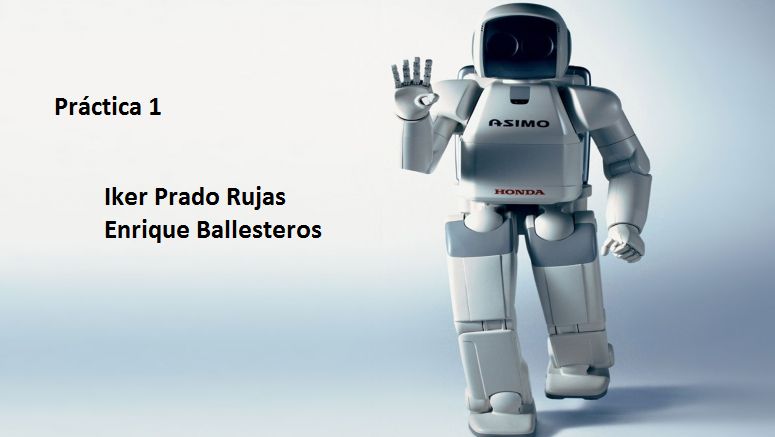
\includegraphics[width=\textwidth]{robotHonda.png}}
\end{center}

\newpage
\textbf{{AIMA}}


\begin{section}{AimaDemoApp }


\end{section}

\newpage
\begin{section}{Puzle de 8}

	
\end{section}

\begin{section}{Mapa desde Arad a Bucharest}


\end{section}


\begin{section}{SearchDemoOsmAgentApp }


\end{section}


\begin{section}{Librerías y definiciones de estado para el puzzle de 8 }


\end{section}


\begin{section}{Librerías y definiciones de estado para el mapa }


\end{section}

\end{document}

